\documentclass[xcolor={usenames,dvipsnames,svgnames}, compress]{beamer}

\usepackage{booktabs}
\usepackage{dcolumn}
\usepackage{colortbl}
\usepackage{xcolor}
\usepackage{hyperref}
\usepackage{amsmath}
\usepackage{wrapfig}
\usepackage{algorithm}
\usepackage[noend]{algpseudocode} 
\usepackage{pifont}
\usepackage[style=authoryear-comp]{biblatex}
\usepackage{marvosym}
\usepackage{mathtools}
\usepackage{array}
\usepackage[export]{adjustbox}


\usepackage[font=scriptsize]{caption}


% 
% custom colors
\definecolor{untractable_red}{RGB}{209, 25, 25}
\definecolor{tractable_green}{RGB}{0, 153, 51}

\newcommand{\argmax}{\operatornamewithlimits{argmax}}
\newcommand{\argmin}{\operatornamewithlimits{argmin}}
\newcommand{\nodeset}[1]{\bm{\mathsf{#1}}}

\newcolumntype{R}[2]{
  >{\adjustbox{angle=#1,lap=\width-(#2)}\bgroup}
  l
  <{\egroup}
}

\newcommand*\rot{\multicolumn{1}{R{45}{1em}}}


\definecolor{lacamgreen} {RGB} {72, 175, 115}
\definecolor{lacamlilac} {RGB} {107,93,153}
\definecolor{lacamlilac2} {RGB} {93, 109, 152}
\definecolor{lacamlightlilac} {RGB} {174, 166, 201}
\definecolor{lacamdarklilac} {RGB} {51, 10, 102}
\definecolor{lacamgold} {RGB} {255, 87, 0}
\definecolor{lacamdarklilac5} {RGB} {51, 10, 102}
\definecolor{lacamgold5} {RGB} {255, 87, 0}
\definecolor{violet} {RGB} {119, 111, 178}
\definecolor{petroil2} {RGB} {36, 165, 175}
\definecolor{petroil4} {RGB} {30, 132, 149}
\definecolor{petroil6} {RGB} {23, 101, 115}
\definecolor{gold2} {RGB} {255, 130, 0}
\definecolor{gold4} {RGB} {250, 100, 0}
\definecolor{gold6} {RGB} {245, 90, 0}

\newcommand{\highlight}[2][yellow]{\mathchoice%
  {\colorbox{#1}{\strut\textcolor{white}{$\displaystyle{#2}$}}}%
  {\colorbox{#1}{\strut\textcolor{white}{$\textstyle{#2}$}}}%
  {\colorbox{#1}{\strut\textcolor{white}{$\scriptstyle{#2}$}}}%
  {\colorbox{#1}{\strut\textcolor{white}{$\scriptscriptstyle{#2}$}}}}%

\newcommand{\highlighttext}[2][yellow]{{\colorbox{#1}{\strut\textcolor{white}{#2}}}}



\usetheme{enziteto}

\setbeamertemplate{headline}{}

\newcommand*\samethanks[1][\value{footnote}]{\footnotemark[#1]}

\makeatletter
\renewcommand*{\@fnsymbol}[1]{\ensuremath{\ifcase#1\or $\Yinyang$\or \dagger\or \ddagger\or
    \mathsection\or \mathparagraph\or \|\or **\or \dagger\dagger
    \or \ddagger\ddagger \else\@ctrerr\fi}}
\makeatother


% 
% custom colors
\definecolor{untractable_red}{RGB}{209, 25, 25}
\definecolor{tractable_green}{RGB}{0, 153, 51}

\newcommand{\cmark}{\ding{51}}%
\newcommand{\xmark}{\ding{55}}

% \bibliographystyle{splncs03}
% \bibliography{../tiselac}

\setbeamertemplate{bibliography item}{\hspace{10pt}\raise .2ex\hbox{\textcolor{lacamlilac}{$\boldsymbol{\oplus}$}}}

\begin{document}

\newlength{\custombulletheight}
\setlength{\custombulletheight}{\dimexpr0.5\ht1-0.5\ht2}

\title{Fast and Accurate Denstity Estimation with Extremely Randomized\\
  Cutset Networks}
\author{Nicola {Di
    Mauro}{\raisebox{2pt}{\hspace{2pt}
\includegraphics[width=5pt]{figures/yinyang}}}
  \and \emph{\textbf{Antonio
      Vergari}}{\raisebox{2pt}{\hspace{2pt}
\includegraphics[width=5pt]{figures/yinyang}}}
  \and Teresa M.A. Basile \and Floriana
  Esposito\\\vspace{-10pt}{\flushleft\raisebox{-1pt}{
\includegraphics[width=5pt]{figures/yinyang}}\  =\ \it both authors contributed equally}}
\date{}
% \institute{Department of Computer Science, University of Bari ``Aldo Moro'', Bari, Italy
% \and 
% Department of Physics, University of Bari ``Aldo Moro'', Bari, Italy
% \and
% National Institute for Nuclear Physics (INFN), Bari Division, Bari, Italy
% }
\department{\bf University of Bari\quad ---\quad Department of Computer Science\quad ---\quad Department
    of Physics\\
    LACAM Machine Learning Lab\quad ---\quad National Institute for Nuclear Physics}
%\laboratory{LACAM Laboratory}
%\group{Machine Learning}
\institutelogo{
\includegraphics[width=25pt]{figures/unibaba}
      \hspace{20pt}
      % \vspace{5pt}
      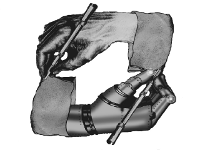
\includegraphics[width=32pt]{figures/lacam}
      \hspace{20pt}
      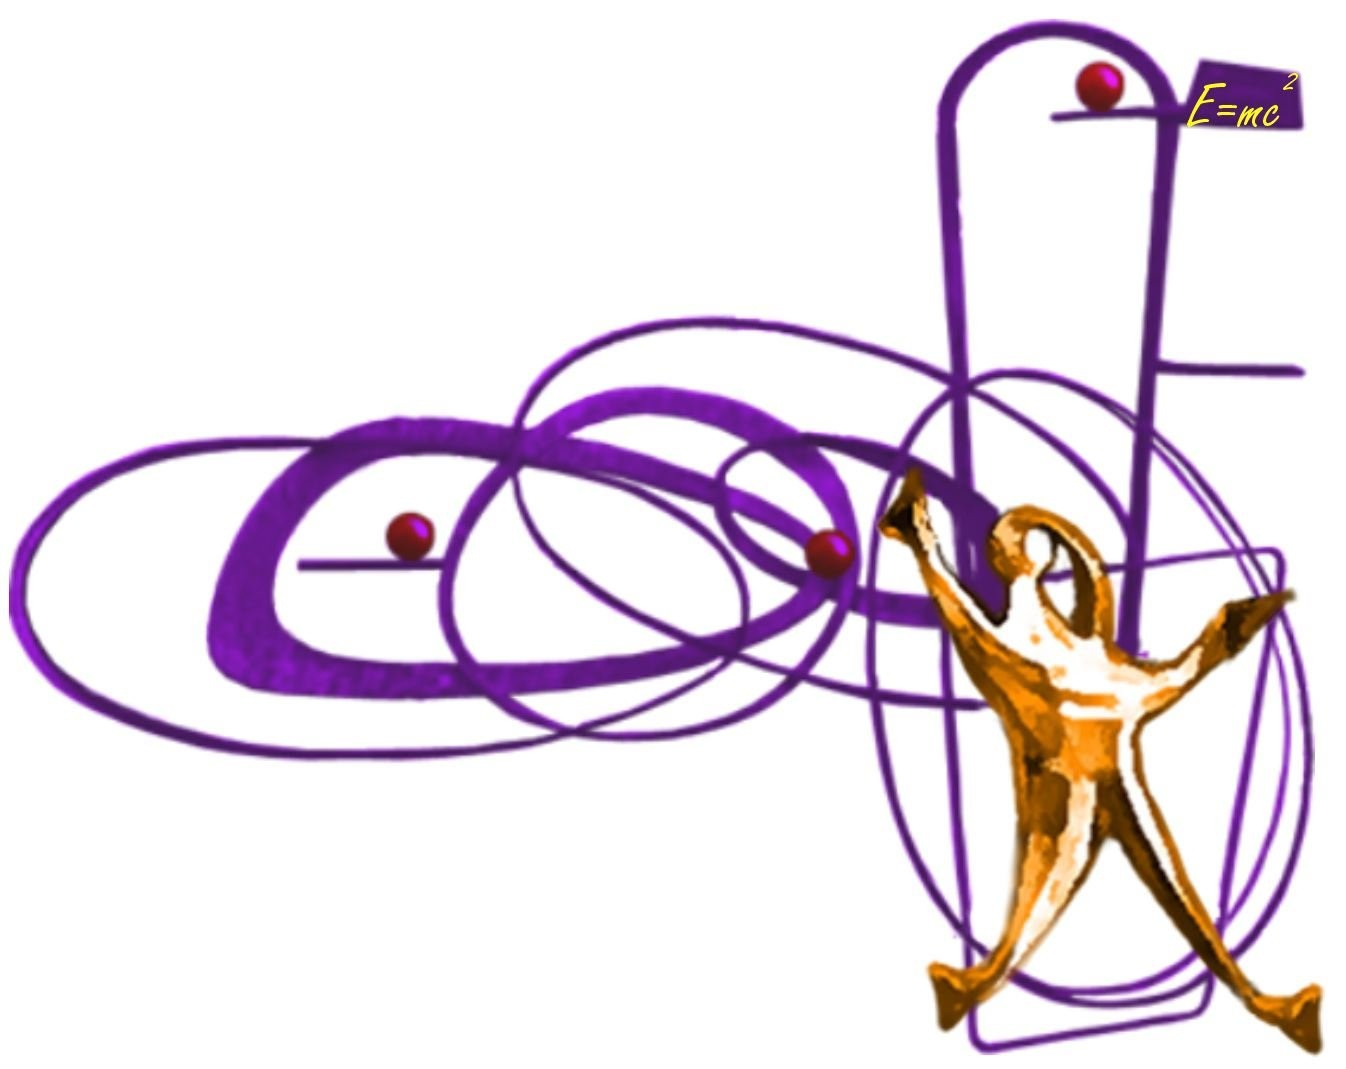
\includegraphics[width=32pt]{figures/fisicalogo}
      \hspace{25pt}
      
\includegraphics[width=22pt]{figures/infn}}
%\lablogo{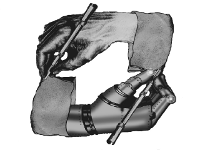
\includegraphics[width=35pt]{figures/lacam}}
\date{19th September - \textbf{ECML-PKDD 2017} - Skopje, Macedonia}

\makeatletter
\defbeamertemplate*{title page}{custom-enziteto}[1][]
{
  \begin{minipage}[t]{0.9\linewidth}
    \vspace{0pt}
    % 
\includegraphics[width=25pt]{Figures/unibaba}
    \ifdefined\@institutelogo
    \@institutelogo
    \fi
  \end{minipage}
  \begin{minipage}[t]{0.9\linewidth}
    \vspace{2pt}
    \flushleft
    {\usebeamerfont{institute}\insertinstitute\par}
    \vspace{2pt}
    \ifdefined\@department
    \tiny\@department
    \fi
  \end{minipage}
  \ifdefined\@laboratory
  %\hspace{10pt}
  \begin{minipage}[t]{0.12\linewidth}
    \vspace{0pt}
    \ifdefined\@lablogo
    \@lablogo
    \else
    \hspace{10pt}
    \fi
  \end{minipage}
  \begin{minipage}[t]{0.40\linewidth}
    \vspace{7pt}
    \flushleft
    \tiny\textbf{\@laboratory}\par
    \vspace{2pt}
    \ifdefined\@group
    \@group
    \fi
  \end{minipage}
  \par
  \fi
  \vspace{15pt}
  
  \Large\usebeamerfont{title}\textcolor{lacamdarklilac5}{\inserttitle}\par%\textcolor{lacamlilac}{\inserttitle}\par
  \vspace{5pt}
  \small\usebeamerfont{subtitle}\textcolor{lacamlilac}{\insertsubtitle}\par
  \vspace{15pt}
  \usebeamerfont{author}\insertauthor\par
  
  \ifdefined\@gliph
  \vspace{7pt}
  \@gliph\par
  \vspace{7pt}
  \else
  \vspace{21pt}
  \fi
  \usebeamerfont{date}\insertdate\par
  
}
\makeatother


{
  \setbeamertemplate{headline}{}
  \setbeamertemplate{footline}{}
  \begin{frame}
    \titlepage
  \end{frame}
}

\begin{frame}[t]
  \frametitle{Outline}
  \bigskip
  $\rightarrow$ \textcolor{lacamlightlilac}{\large\textbf{Density Estimation}}\par
  \bigskip
  $\rightarrow$ \textcolor{lacamlightlilac}{\large\textbf{Tractable
      Probabilistic Models}}\par
  \bigskip
  $\rightarrow$ \textcolor{lacamlightlilac}{\large\textbf{Cutset Networks}}\par
  \bigskip
  $\rightarrow$ \textcolor{lacamlightlilac}{\large\textbf{XCNets}}\par
  \bigskip
  $\rightarrow$ \textcolor{lacamlightlilac}{\large\textbf{Experiments}}\par
  \bigskip
  $\rightarrow$ \textcolor{lacamlightlilac}{\large\textbf{Conclusions}}\par
  \bigskip
  $\rightarrow$ \textcolor{lacamlightlilac}{\large\textbf{\emph{References}}}\par
\end{frame}


\begin{frame}[t]
  \frametitle{Density Estimation}
  \small
  \emph{\textbf{Density estimation}} is the unsupervised task of
    learning an estimator for the joint probability distribution
    $p(\mathbf{X})$ from a set of i.i.d. samples $\mathcal{D}=\{\mathbf
    x^i\}_{i=1}^m$ over random variables (RVs) $\mathbf{X}=\{X_{1},\dots,X_{n}\}$\\[17pt]
    
    Given such an estimator, one uses it to \emph{answer
    probabilistic queries} about configurations on $\mathbf{X}$,
  i.e. to do \emph{\textbf{inference}}.
  E.g., classification can be performed by Most Probable Explanaition
  (MPE) inference: $y^{*}=\argmax_{y\sim Y}p(y|\mathbf{X})$.
  \\[17pt]

    The main challenge in density estimation is balancing:
    \begin{itemize}
      \setlength\itemsep{-3pt}
    \item the \highlighttext[lacamlilac]{\textbf{\emph{representation
            expressiveness}}} of the model to learn
    \item the \highlighttext[gold4]{\textbf{\emph{cost of learning}}}
      such a model
      \item and the \highlighttext[petroil2]{\textbf{\emph{cost of performing inference}}} on it
    \end{itemize}

\end{frame}

\begin{frame}[t]
  \frametitle{Tractable Probabilistic Models (TPMs)}

  \small
  Classical Probabilistic Graphical Models like \emph{\textbf{Bayesian Networks}}
    (\textbf{BNs}) and \emph{\textbf{Markov Networks}} (\textbf{MNs}) are \highlighttext[lacamlilac]{highly expressive} but
    exact \highlighttext[petroil2]{\textbf{inference is generally
        \emph{NP-hard}}} with them~\parencite{Roth1996}.
    %\vspace{20pt}

    \begin{figure}
      \centering
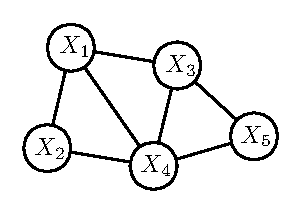
\includegraphics[width=0.3\linewidth]{figures/mrf} \hspace{30pt} 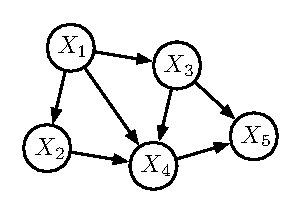
\includegraphics[width=0.3\linewidth]{figures/bn}      
    \end{figure}
\vspace{-5pt}
    \emph{\textbf{Tractable Probabilistic Models} }  (\textbf{TPMs})
    on the other hand, are density estimators for which some kind of  \highlighttext[petroil2]{\textbf{\emph{exact}} \textbf{inference is}
    \textbf{\emph{tractable}}}, i.e. \emph{polynomial} in the number
  of RVs, i.e., $n$, or their
    domains\par
    \hfill$\rightarrow$ \highlighttext[gold4]{learning may still be hard to scale on
    high-dimensional data}\\[20pt]

  
  \end{frame}

  \begin{frame}[t]
    \frametitle{Product of Bernoullis (PoBs)}

    A not so much expressive TPM, assuming all RVs to be independent:
    
    \begin{figure}
      \centering
      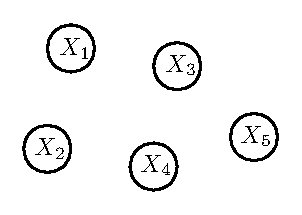
\includegraphics[width=0.3\linewidth]{figures/nf}
    \end{figure}\vspace{-5pt}
    $$\highlight[lacamlilac]{\mathsf{p}(\mathbf{x}) =\prod\nolimits_{i=1}^{n}\mathsf{p}(x_{i})}$$\vspace{5pt}

    Learning a PoB has linear time complexity
    $\highlight[gold4]{O(nm)}$\par
    Complete evidence inference is linear $\highlight[petroil2]{O(n)}$\par
    
  \end{frame}


  \begin{frame}[t]
    \frametitle{Chow-Liu Trees (CLTrees)}
\small
    A \emph{directed tree-structured model}~\parencite{Meila2000} over
    $\mathbf{X}$ is a BN in which each node $X_{i}\in\mathbf{X}$ has at most one
    parent, $\mathrm{Pa}_{X_i}$.
    \begin{figure}
      \centering
      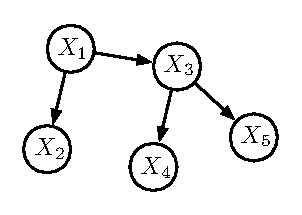
\includegraphics[width=0.3\linewidth]{figures/clt}
    \end{figure}\vspace{-5pt}
    $$\highlight[lacamlilac]{\mathsf{p}(\mathbf{x}) =
    \prod\nolimits_{i=1}^n\mathsf{p}(x_i|\mathrm{Pa}_{x_i})}$$\vspace{5pt}

    Complete evidence inference is still linear for \textsf{CLtrees}: $\highlight[petroil2]{O(n)}$\par
    But learning now  takes  quadratic time $\highlight[gold4]{O(n^2(m + \log n))}$\par
  \end{frame}


\begin{frame}[t]
  \frametitle{Cutset Networks (CNets)}
  \footnotesize
  \vspace{-10pt}
  \begin{figure}
     \centering
     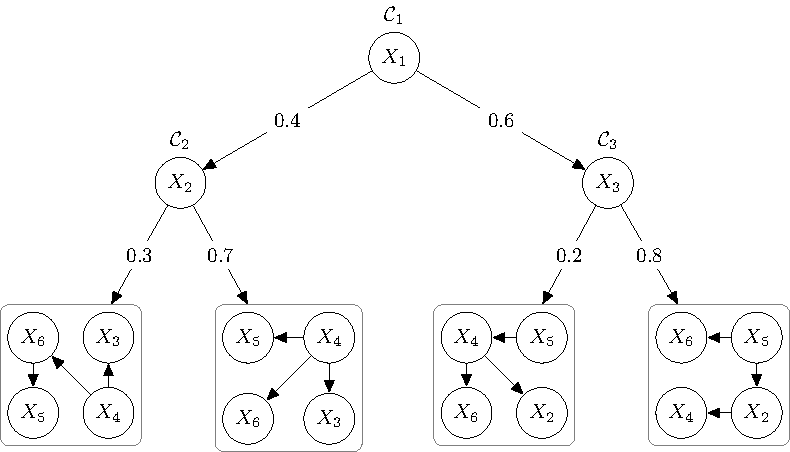
\includegraphics[width=7cm]{figures/csn}
     % \caption{\scriptsize }
  \label{fig:csn}
\end{figure}
\vspace{-10pt}
  A \emph{\textbf{Cutset Network}} (CNet) $\mathcal{C}$ is a TPM represented via a
  \textbf{weighted probabilistic model} tree over $\mathbf{X}$ 
    recursively defined as: % \textbf{(I)} a TPM $\mathcal{M}$, with
    %   scope $\mathbf{X}$ (\emph{leaf}) or \textbf{(II)} a weighted  disjunction (OR node) of two CNets $\mathcal C_0$ and $\mathcal C_1$
    %  conditioned on RV $X_i \in \mathbf X$,  with
    % weights $w_i^0$ and $w_i^1$ s.t. $w_i^0 + w_i^1 = 1$,
    % where $\mathsf{scope}(\mathcal C_{0})=\mathsf{scope}(\mathcal C_{1})=\mathbf X_{\setminus i}$
    \begin{enumerate}
    \item a TPM $\mathcal{M}$  , with
       $\mathsf{scope}(\mathcal{M})=\mathbf X$
      \item a weighted  disjunction (OR node) of two CNets $\mathcal C_0$ and $\mathcal C_1$
     conditioned on RV $X_i \in \mathbf X$,  with
    weights $w_i^0$ and $w_i^1$ s.t. $w_i^0 + w_i^1 = 1$,
    where $\mathsf{scope}(\mathcal C_{0})=\mathsf{scope}(\mathcal C_{1})=\mathbf X_{\setminus i}$
    \end{enumerate}
    
  \end{frame}
\begin{frame}[t]
  \frametitle{CNets I}
  \small
  \begin{figure}
     \centering
     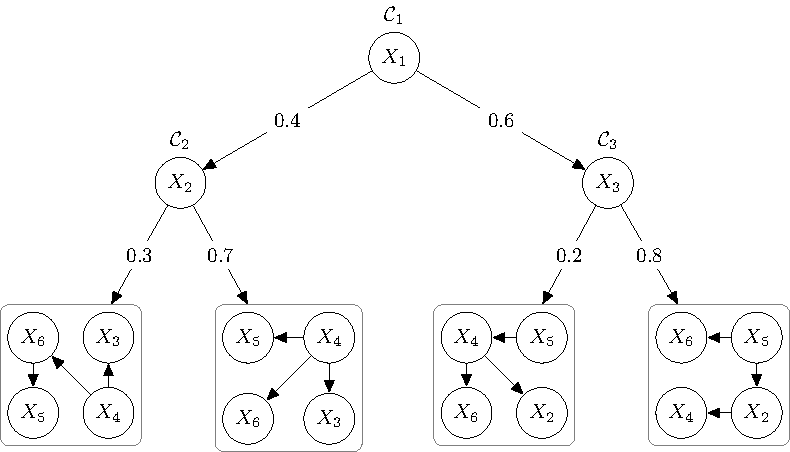
\includegraphics[width=7cm]{figures/csn}
     % \caption{\scriptsize }
  \label{fig:csn}
\end{figure}
  A CNet $\mathcal{C}$ defines the following joint distribution:
  \begin{equation*}
\highlight[lacamlilac]{\mathsf{p}(\mathbf{x}) = \mathsf{p}_l(\mathbf
x_{|\mathsf{scope}(\mathcal C)\setminus \mathsf{scope}(\mathcal
  M_l)})\mathsf{p}_{\mathcal M_l}(\mathbf x_{| \mathsf{scope}(\mathcal
  M_l)})}\label{eq:cnetdistr}
\end{equation*}
    % % recursively defined as:
    % \begin{enumerate}
    % \item a TPM $\mathcal{M}$, with
    %   $\mathsf{scope}(\mathcal{M})=\mathbf X$
    %   \item a weighted  disjunction (OR node) of two CNets $\mathcal C_0$ and $\mathcal C_1$
    %  conditioned on RV $X_i \in \mathbf X$,  with
    % weights $w_i^0$ and $w_i^1$ s.t. $w_i^0 + w_i^1 = 1$,
    % where $\mathsf{scope}(\mathcal C_{0})=\mathsf{scope}(\mathcal C_{1})=\mathbf X_{\setminus i}$
    % \end{enumerate}
    
  \end{frame}

  \begin{frame}[t]
  \frametitle{CNets II}
  \small
  \begin{figure}
     \centering
     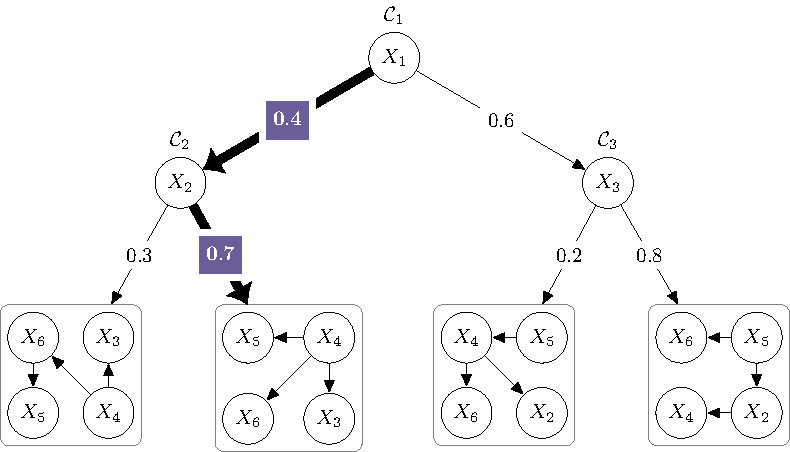
\includegraphics[width=7cm]{figures/csn-II}
     % \caption{\scriptsize }
  \label{fig:csn}
\end{figure}
  A CNet $\mathcal{C}$ acts as a \emph{\textbf{deterministic mixture of experts}} in
  which the OR tree acts as the \textbf{gating function}
  \begin{equation*}
\mathsf{p}(\mathbf{x}) = \highlight[lacamlilac]{\mathsf{p}_l(\mathbf
x_{|\mathsf{scope}(\mathcal C)\setminus \mathsf{scope}(\mathcal
  M_l)})}\mathsf{p}_{\mathcal M_l}(\mathbf x_{| \mathsf{scope}(\mathcal
  M_l)})\label{eq:cnetdistr}
\end{equation*}
    % recursively defined as:
    % \begin{enumerate}
    % \item a TPM $\mathcal{M}$, with
    %   $\mathsf{scope}(\mathcal{M})=\mathbf X$
    %   \item a weighted  disjunction (OR node) of two CNets $\mathcal C_0$ and $\mathcal C_1$
    %  conditioned on RV $X_i \in \mathbf X$,  with
    % weights $w_i^0$ and $w_i^1$ s.t. $w_i^0 + w_i^1 = 1$,
    % where $\mathsf{scope}(\mathcal C_{0})=\mathsf{scope}(\mathcal C_{1})=\mathbf X_{\setminus i}$
    % \end{enumerate}
    
\end{frame}

\begin{frame}[t]
  \frametitle{CNets III}
  \small
  \begin{figure}
     \centering
     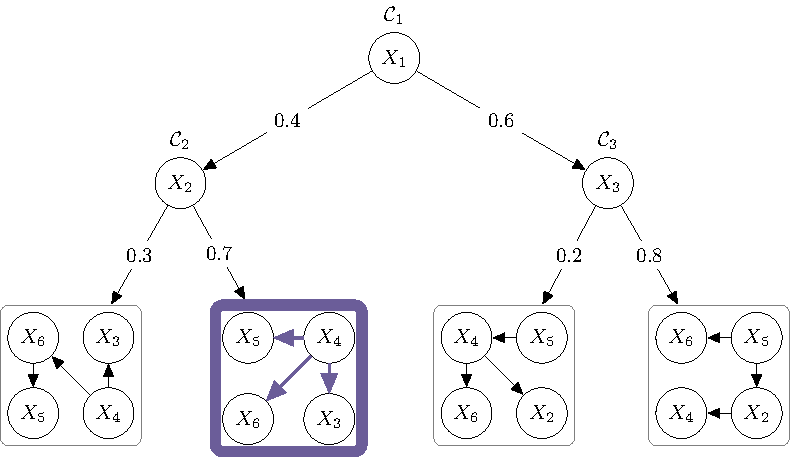
\includegraphics[width=7cm]{figures/csn-III}
     % \caption{\scriptsize }
  \label{fig:csn}
\end{figure}
  and in which leaf models $\mathcal{M}_{l}$ play the role of \textbf{local
  experts}\vspace{-10pt}
  \begin{equation*}
\mathsf{p}(\mathbf{x}) = \mathsf{p}_l(\mathbf
x_{|\mathsf{scope}(\mathcal C)\setminus \mathsf{scope}(\mathcal
  M_l)})\highlight[lacamlilac]{\mathsf{p}_{\mathcal M_l}(\mathbf x_{| \mathsf{scope}(\mathcal
  M_l)})}\label{eq:cnetdistr}
\end{equation*}\vspace{-20pt}
complete evidence inference is still linear $\highlight[petroil2]{O(n)}$!

    % recursively defined as:
    % \begin{enumerate}
    % \item a TPM $\mathcal{M}$, with
    %   $\mathsf{scope}(\mathcal{M})=\mathbf X$
    %   \item a weighted  disjunction (OR node) of two CNets $\mathcal C_0$ and $\mathcal C_1$
    %  conditioned on RV $X_i \in \mathbf X$,  with
    % weights $w_i^0$ and $w_i^1$ s.t. $w_i^0 + w_i^1 = 1$,
    % where $\mathsf{scope}(\mathcal C_{0})=\mathsf{scope}(\mathcal C_{1})=\mathbf X_{\setminus i}$
    % \end{enumerate}
    
\end{frame}

\begin{frame}[t]
  \frametitle{Learning CNets I}
  \small
      \textbf{Top-down greedy} CNet learners %~\cite{Rahman2014,DiMauro2015a}
    can be unified in single template, $\mathsf{LearnCNet}$:\vspace{-10pt}
 \begin{center}  
  \begin{minipage}{0.9\linewidth}
    \vspace{10pt}
        \scriptsize
        {\hrule\flushleft\textsf{LearnCNet}($\mathcal{D}$, $\mathbf{X}$, 
        $\delta$, $\sigma$)\\\hrule}
        % \blindtext
%\begin{algorithm}
%  \caption{\textsf{\textsf{LearnCNet}}($\mathcal{D}$, $\mathbf{X}$, $\alpha$, $\delta$, $\sigma$)}
%  \label{algo:learn-cnet}
  \begin{algorithmic}[1]
    \State \textbf{Input:} a dataset $\mathcal{D}$ over RVs
    $\mathbf{X}$; $\delta$
    min number samples; $\sigma$ min number features
    \State  \textbf{Output:}  a CNet $\mathcal{C}$ encoding  $\mathsf{p}_{\mathcal{C}}(\mathbf{X})$ learned from $\mathcal D$
    \If {$|\mathcal D|>\delta$ \textbf{and} $|\mathbf X|>\sigma$}
    \State $X_i\leftarrow  \mathsf{select}(\mathcal D, \mathbf X)$
    % \If {$\mathsf{success}$}
    %\Comment {select the RV to condition on}
    \State $\mathcal D_0 \leftarrow \{\xi \in \mathcal D: \xi[X_i]=0 \}$, $\mathcal D_1 \leftarrow \{\xi \in \mathcal D: \xi[X_i]=1 \}$
    \State $w_0 \leftarrow |\mathcal D_0| / |\mathcal D|$, $w_1 \leftarrow |\mathcal   D_1| / |\mathcal D|$
    \State $\mathcal{C} \leftarrow
    w_0\cdot\mathsf{LearnCNet}(\mathcal D_0, \mathbf X_{\setminus i},
     \delta, \sigma) + w_1 \cdot\mathsf{LearnCNet}(\mathcal D_1, \mathbf X_{\setminus i}, \delta, \sigma) $
    % \Else 
    % \State $C \leftarrow \mathcal T$ 
    %\EndIf
    \Else 
    \State $\mathcal{C} \leftarrow
    \highlight[gold4]{\mathsf{learnLeafDistribution}(\mathcal D,
      \mathbf X
      )}$
    \Comment {Grow a leaf TPM}
    \EndIf
    \State \Return $\mathcal{C}$
  \end{algorithmic}
  \hrule
\end{minipage}
\end{center}
\vspace{10pt}
  \small
  in which for the base case, if no conditioning is possible, \emph{a leaf
  distribution is estimated}
\end{frame}

\begin{frame}[t]
  \frametitle{Learning CNets II}
  \small
      \textbf{Top-down greedy} CNet learners %~\cite{Rahman2014,DiMauro2015a}
    can be unified in single template, $\mathsf{LearnCNet}$:\vspace{-10pt}
 \begin{center}  
  \begin{minipage}{0.9\linewidth}
    \vspace{10pt}
        \scriptsize
        {\hrule\flushleft\textsf{LearnCNet}($\mathcal{D}$, $\mathbf{X}$, $\alpha$,
        $\delta$, $\sigma$)\\\hrule}
        % \blindtext
%\begin{algorithm}
%  \caption{\textsf{\textsf{LearnCNet}}($\mathcal{D}$, $\mathbf{X}$, $\alpha$, $\delta$, $\sigma$)}
%  \label{algo:learn-cnet}
  \begin{algorithmic}[1]
    \State \textbf{Input:} a dataset $\mathcal{D}$ over RVs $\mathbf{X}$;  $\delta$
    min number samples; $\sigma$ min number features
    \State  \textbf{Output:}  a CNet $\mathcal{C}$ encoding  $\mathsf{p}_{\mathcal{C}}(\mathbf{X})$ learned from $\mathcal D$
    \If {$|\mathcal D|>\delta$ \textbf{and} $|\mathbf X|>\sigma$}
    \State $X_i\leftarrow  \highlight[gold4]{\mathsf{select}(\mathcal D, \mathbf X)}$
    % \If {$\mathsf{success}$}
    \Comment {select the RV to condition on}
    \State $\mathcal D_0 \leftarrow \{\xi \in \mathcal D: \xi[X_i]=0 \}$, $\mathcal D_1 \leftarrow \{\xi \in \mathcal D: \xi[X_i]=1 \}$
    \State $w_0 \leftarrow |\mathcal D_0| / |\mathcal D|$, $w_1 \leftarrow |\mathcal   D_1| / |\mathcal D|$
    \State $\mathcal{C} \leftarrow
    w_0\cdot\mathsf{LearnCNet}(\mathcal D_0, \mathbf X_{\setminus i},
     \delta, \sigma) + w_1 \cdot\mathsf{LearnCNet}(\mathcal D_1, \mathbf X_{\setminus i}, \delta, \sigma) $
    % \Else 
    % \State $C \leftarrow \mathcal T$ 
    %\EndIf
    \Else 
    \State $\mathcal{C} \leftarrow \mathsf{learnLeafDistribution}(\mathcal D, \mathbf X)$
    \EndIf
    \State \Return $\mathcal{C}$
  \end{algorithmic}
  \hrule
\end{minipage}
\end{center}
\vspace{10pt}
  \small
  or selecting a RV to condition on is performed, splitting the
  dataset and recursing
\end{frame}




\begin{frame}[t]
  \frametitle{Learning CNets III}
  \small

  \highlighttext[gold4]{Different implementations of \textsf{select}}
  lead to different time complexities:
  \begin{center}
      \begin{minipage}{0.9\linewidth}
        \begin{description}[align=parright]
        \item[\textbf{\textsf{entCNet}}] choosing
          $X_{i}$ to lower approximate average joint entropy~\parencite{Rahman2014}\par
          {\hfill $\rightarrow\highlight[gold4]{O(mn^2)}$}
        \item[\textbf{\textsf{dCSN}}] choosing
          $X_{i}$ in a principled way improving likelihood~\parencite{DiMauro2015a}\par
          {\hfill $\rightarrow$ $\highlight[gold4]{O(n^3(m + \log n))}$}
        \end{description}
      \end{minipage}
    \end{center}

  \vspace{10pt}
  Quadratic and cubic times for \emph{each} RV selection do not scale
  on high dimensional data \hspace{80pt}$\rightarrow$
  We aim at drastically reducing it!
\end{frame}

\begin{frame}[t]
  \frametitle{XCNets I}
\small
  \emph{\textbf{XCNets}} (\textbf{Extremely Randomized CNets}) are CNets built by \textsf{LearnCNet} when
    \textsf{\textbf{select}} chooses one RV \emph{completely at random}.\par
    {\hfill\textsf{select} time complexity $\rightarrow$ $\highlight[gold4]{O(1)}$!}
    \vspace{20pt}

    Advantages of a \textbf{single} XCNet over a classically learned CNet:
    \begin{itemize}
      \setlength{\itemsep}{-3pt}
      \item \highlighttext[gold4]{extremely fast} to learn
    \item only \highlighttext[lacamlilac]{slightly less accurate} as density estimators
    \item almost as good at generating samples
    \item less prone to overfitting
    % \item leading to fast and state-of-the-art estimators  when put in ensembles 
    \end{itemize}
\vspace{20pt}

When plugged into \textbf{ensembles} they outperform state-of-the-art
density estimators in a fraction of the time!
\end{frame}

\begin{frame}[t]
  \frametitle{XCNets II}
\small

Why a single XCNet is \emph{not much worse} than a CNet?\\[10pt]

Because of the mixture of experts interpretations, a path $p=p_{(1)}p_{(2)}\cdots p_{(k)}$ connects the root to a
    single leaf $\mathcal{M}_{l}$ after observing $x_{1} x_{2} \cdots  x_{k}$,
$\mathsf{p}_l(\mathbf x_{|\mathsf{sc}(\mathcal C)\setminus
  \mathsf{sc}(\mathcal M_l)})$ is decomposed by the chain rule across
path $p$ \par
{\hfill$\rightarrow$  \highlighttext[petroil2]{shuffling
  $X_{p_(0)},\dots,X_{p_{k}}$ does not influence inference!}}\\[10pt]

Focus on learning \highlighttext[lacamlilac]{\emph{\textbf{accurate
      local experts}}} (leaves) than the gating function!
Sampling is less affected:
    \begin{figure}[t]
  \centering
  \setlength{\tabcolsep}{0pt}
  \renewcommand{\arraystretch}{0}
  \newcolumntype{S}{>{\centering\arraybackslash} m{.04\linewidth} }
  \newcolumntype{X}{>{\centering\arraybackslash} m{.028\linewidth} }
\begin{tabular}{SSSSSXSSSSSXSSSSSXSSSSS}
 
\includegraphics[width=\linewidth]{{figures/mnist.cnet.50.0}.pdf}
& 
\includegraphics[width=\linewidth]{{figures/mnist.cnet.50.1}.pdf}
& 
\includegraphics[width=\linewidth]{{figures/mnist.cnet.50.2}.pdf}
& 
\includegraphics[width=\linewidth]{{figures/mnist.cnet.50.3}.pdf}
& 
\includegraphics[width=\linewidth]{{figures/mnist.cnet.50.5}.pdf}
&
& 
\includegraphics[width=\linewidth]{{figures/mnist.cnet.near.50.0}.pdf}
& 
\includegraphics[width=\linewidth]{{figures/mnist.cnet.near.50.1}.pdf}
& 
\includegraphics[width=\linewidth]{{figures/mnist.cnet.near.50.2}.pdf}
& 
\includegraphics[width=\linewidth]{{figures/mnist.cnet.near.50.3}.pdf}
& 
\includegraphics[width=\linewidth]{{figures/mnist.cnet.near.50.5}.pdf}
&    
& 
\includegraphics[width=\linewidth]{{figures/mnist.xcnet.50.1}.pdf}
& 
\includegraphics[width=\linewidth]{{figures/mnist.xcnet.50.2}.pdf}
& 
\includegraphics[width=\linewidth]{{figures/mnist.xcnet.50.3}.pdf}
& 
\includegraphics[width=\linewidth]{{figures/mnist.xcnet.50.4}.pdf}
& 
\includegraphics[width=\linewidth]{{figures/mnist.xcnet.50.5}.pdf}
&
& 
\includegraphics[width=\linewidth]{{figures/mnist.xcnet.near.50.1}.pdf}
& 
\includegraphics[width=\linewidth]{{figures/mnist.xcnet.near.50.2}.pdf}
& 
\includegraphics[width=\linewidth]{{figures/mnist.xcnet.near.50.3}.pdf}
& 
\includegraphics[width=\linewidth]{{figures/mnist.xcnet.near.50.4}.pdf}
& 
\includegraphics[width=\linewidth]{{figures/mnist.xcnet.near.50.5}.pdf}\\

 
\includegraphics[width=\linewidth]{{figures/mnist.cnet.50.6}.pdf}
& 
\includegraphics[width=\linewidth]{{figures/mnist.cnet.50.7}.pdf}
& 
\includegraphics[width=\linewidth]{{figures/mnist.cnet.50.8}.pdf}
& 
\includegraphics[width=\linewidth]{{figures/mnist.cnet.50.9}.pdf}
& 
\includegraphics[width=\linewidth]{{figures/mnist.cnet.50.11}.pdf}
&
& 
\includegraphics[width=\linewidth]{{figures/mnist.cnet.near.50.6}.pdf}
& 
\includegraphics[width=\linewidth]{{figures/mnist.cnet.near.50.7}.pdf}
& 
\includegraphics[width=\linewidth]{{figures/mnist.cnet.near.50.8}.pdf}
& 
\includegraphics[width=\linewidth]{{figures/mnist.cnet.near.50.9}.pdf}
& 
\includegraphics[width=\linewidth]{{figures/mnist.cnet.near.50.11}.pdf}
&  
& 
\includegraphics[width=\linewidth]{{figures/mnist.xcnet.50.6}.pdf}
& 
\includegraphics[width=\linewidth]{{figures/mnist.xcnet.50.8}.pdf}
& 
\includegraphics[width=\linewidth]{{figures/mnist.xcnet.50.9}.pdf}
& \includegraphics[width=\linewidth]{{figures/mnist.xcnet.50.10}.pdf}
& \includegraphics[width=\linewidth]{{figures/mnist.xcnet.50.11}.pdf}
&
& \includegraphics[width=\linewidth]{{figures/mnist.xcnet.near.50.6}.pdf}
& \includegraphics[width=\linewidth]{{figures/mnist.xcnet.near.50.8}.pdf}
& \includegraphics[width=\linewidth]{{figures/mnist.xcnet.near.50.9}.pdf}
& \includegraphics[width=\linewidth]{{figures/mnist.xcnet.near.50.10}.pdf}
& \includegraphics[width=\linewidth]{{figures/mnist.xcnet.near.50.11}.pdf}\\
 
 \includegraphics[width=\linewidth]{{figures/mnist.cnet.50.12}.pdf}
& \includegraphics[width=\linewidth]{{figures/mnist.cnet.50.13}.pdf}
& \includegraphics[width=\linewidth]{{figures/mnist.cnet.50.14}.pdf}
& \includegraphics[width=\linewidth]{{figures/mnist.cnet.50.15}.pdf}
& \includegraphics[width=\linewidth]{{figures/mnist.cnet.50.17}.pdf}
&
& \includegraphics[width=\linewidth]{{figures/mnist.cnet.near.50.12}.pdf}
& \includegraphics[width=\linewidth]{{figures/mnist.cnet.near.50.13}.pdf}
& \includegraphics[width=\linewidth]{{figures/mnist.cnet.near.50.14}.pdf}
& \includegraphics[width=\linewidth]{{figures/mnist.cnet.near.50.15}.pdf}
& \includegraphics[width=\linewidth]{{figures/mnist.cnet.near.50.17}.pdf}
&
&  \includegraphics[width=\linewidth]{{figures/mnist.xcnet.50.12}.pdf}
& \includegraphics[width=\linewidth]{{figures/mnist.xcnet.50.13}.pdf}
& \includegraphics[width=\linewidth]{{figures/mnist.xcnet.50.14}.pdf}
& \includegraphics[width=\linewidth]{{figures/mnist.xcnet.50.16}.pdf}
& \includegraphics[width=\linewidth]{{figures/mnist.xcnet.50.17}.pdf}
&
& \includegraphics[width=\linewidth]{{figures/mnist.xcnet.near.50.12}.pdf}
& \includegraphics[width=\linewidth]{{figures/mnist.xcnet.near.50.13}.pdf}
& \includegraphics[width=\linewidth]{{figures/mnist.xcnet.near.50.14}.pdf}
& \includegraphics[width=\linewidth]{{figures/mnist.xcnet.near.50.16}.pdf}
& \includegraphics[width=\linewidth]{{figures/mnist.xcnet.near.50.17}.pdf}\\

 \includegraphics[width=\linewidth]{{figures/mnist.cnet.50.18}.pdf}
& \includegraphics[width=\linewidth]{{figures/mnist.cnet.50.19}.pdf}
& \includegraphics[width=\linewidth]{{figures/mnist.cnet.50.20}.pdf}
& \includegraphics[width=\linewidth]{{figures/mnist.cnet.50.21}.pdf}
& \includegraphics[width=\linewidth]{{figures/mnist.cnet.50.23}.pdf}
&
& \includegraphics[width=\linewidth]{{figures/mnist.cnet.near.50.18}.pdf}
& \includegraphics[width=\linewidth]{{figures/mnist.cnet.near.50.19}.pdf}
& \includegraphics[width=\linewidth]{{figures/mnist.cnet.near.50.20}.pdf}
& \includegraphics[width=\linewidth]{{figures/mnist.cnet.near.50.21}.pdf}
& \includegraphics[width=\linewidth]{{figures/mnist.cnet.near.50.23}.pdf}
&
& \includegraphics[width=\linewidth]{{figures/mnist.xcnet.50.18}.pdf}
& \includegraphics[width=\linewidth]{{figures/mnist.xcnet.50.19}.pdf}
& \includegraphics[width=\linewidth]{{figures/mnist.xcnet.50.20}.pdf}
& \includegraphics[width=\linewidth]{{figures/mnist.xcnet.50.22}.pdf}
& \includegraphics[width=\linewidth]{{figures/mnist.xcnet.50.23}.pdf}
&
& \includegraphics[width=\linewidth]{{figures/mnist.xcnet.near.50.18}.pdf}
& \includegraphics[width=\linewidth]{{figures/mnist.xcnet.near.50.19}.pdf}
& \includegraphics[width=\linewidth]{{figures/mnist.xcnet.near.50.20}.pdf}
& \includegraphics[width=\linewidth]{{figures/mnist.xcnet.near.50.22}.pdf}
& \includegraphics[width=\linewidth]{{figures/mnist.xcnet.near.50.23}.pdf}\\

 \includegraphics[width=\linewidth]{{figures/mnist.cnet.50.24}.pdf}
& \includegraphics[width=\linewidth]{{figures/mnist.cnet.50.25}.pdf}
& \includegraphics[width=\linewidth]{{figures/mnist.cnet.50.26}.pdf}
& \includegraphics[width=\linewidth]{{figures/mnist.cnet.50.27}.pdf}
& \includegraphics[width=\linewidth]{{figures/mnist.cnet.50.29}.pdf}
&
& \includegraphics[width=\linewidth]{{figures/mnist.cnet.near.50.24}.pdf}
& \includegraphics[width=\linewidth]{{figures/mnist.cnet.near.50.25}.pdf}
& \includegraphics[width=\linewidth]{{figures/mnist.cnet.near.50.26}.pdf}
& \includegraphics[width=\linewidth]{{figures/mnist.cnet.near.50.27}.pdf}
& \includegraphics[width=\linewidth]{{figures/mnist.cnet.near.50.29}.pdf}
&
& \includegraphics[width=\linewidth]{{figures/mnist.xcnet.50.24}.pdf}
& \includegraphics[width=\linewidth]{{figures/mnist.xcnet.50.25}.pdf}
& \includegraphics[width=\linewidth]{{figures/mnist.xcnet.50.26}.pdf}
& \includegraphics[width=\linewidth]{{figures/mnist.xcnet.50.27}.pdf}
& \includegraphics[width=\linewidth]{{figures/mnist.xcnet.50.29}.pdf}
&
& \includegraphics[width=\linewidth]{{figures/mnist.xcnet.near.50.24}.pdf}
& \includegraphics[width=\linewidth]{{figures/mnist.xcnet.near.50.25}.pdf}
& \includegraphics[width=\linewidth]{{figures/mnist.xcnet.near.50.26}.pdf}
& \includegraphics[width=\linewidth]{{figures/mnist.xcnet.near.50.27}.pdf}
& \includegraphics[width=\linewidth]{{figures/mnist.xcnet.near.50.29}.pdf}\\\\\\
&
&\tiny CNet
&
&
&
&
&
&\tiny Train
&
&
&
&
&
&\tiny XCNet
&
&
&
&
&
&\tiny Train\\  

\end{tabular}

% \caption{Samples obtained from a CNet (a), resp. XCNet (c), learned on 
%   samples of the binarized \texttt{MNIST} dataset, and their nearest neighbor in training set (b), resp. (d).} 
\label{fig:vis}
\end{figure}
% \hspace{50pt}
% \begin{minipage}{0.8\linewidth}
%   \vspace{-20pt}
% \scriptsize  Samples obtained from a CNet (a), resp. XCNet (c), learned on 
%    a binarized version of \texttt{MNIST}, and their nearest neighbor in training set (b), resp. (d).
%  \end{minipage}

 \end{frame}

% \begin{frame}[t]
%   \frametitle{Mixture of Experts}

%   A single CNet can be seen as a peculiar \highlighttext[lacamlilac]{\textbf{\emph{mixture of experts}}}: the OR
%     tree plays as a \emph{deterministic gating function} and leaf distributions
%     as \emph{local experts}.
%     A path $p=p_{(1)}p_{(2)}\cdots p_{(k)}$ connects the root to a
%     single leaf $\mathcal{M}_{l}$ after observing $x_{1} x_{2} \cdots  x_{k}$,
%      Equation~\ref{eq:cnetdistr}.

% $\mathsf{p}_l(\mathbf x_{|\mathsf{sc}(\mathcal C)\setminus
%   \mathsf{sc}(\mathcal M_l)})$ is decomposed by the chain rule across
% path $p$ .\par
% {\hfill$\rightarrow$ randomly shuffling
%   $X_{p_(0)},\dots,X_{p_{k}}$ does not influence inference!}
% \end{frame}

\begin{frame}[t]
  \frametitle{XCNets III}
  \small
  Single CNets learned with $\mathsf{LearnCNet}$ are prone to
  overfitting.\par
  \textbf{\emph{Randomizing the gating function}} in \textsf{XCNets} alleviates this issue.
   \vspace{10pt} 
\begin{figure}[t]
  %\caption{Negative log-likelihood during learning CNets and XCNets.}
  \label{fig:ll}
  \centering
  %\begin{tabular}{ccc}
    \includegraphics[width=0.42\linewidth]{figures/kdd-crop} \hspace{20pt}
    %\includegraphics[width=0.33\linewidth]{figures/msweb-crop} &
    \includegraphics[width=0.41\linewidth]{figures/tmovie-crop}
  %\end{tabular}
\end{figure}
\hspace{30pt}
\begin{minipage}{0.8\linewidth}
  \vspace{-10pt}
\tiny  Learning curves of CNets and XCNets (negative
log-likelihoods) on $\mathsf{KddCup2k}$ and $\mathsf{EachMovie}$
The latter overfits much later than the former.
\end{minipage}\par
\vspace{10pt}
Moreover, it helps \textbf{differentiating the local leaf experts }
\end{frame}

\begin{frame}[t]
  \frametitle{Ensembles of XCNets}
  \small

  
  Ensembles of XCNets do not require to additionally
  diversify each component (e.g. no bootstrapping required).\\[10pt]

  Learning up to \textbf{500 components} of XCNets is still \textbf{faster
than learning 40} models of other variants:

\vspace{10pt}

    \begin{center}
      \begin{minipage}{0.9\linewidth}
        \begin{description}[align=parright]
        \item[\textbf{\textsf{CNet}}$_{\mathsf{bag}}$]
          bagging \textsf{entCSN}~\parencite{Rahman2016a}\par
          %{\hfill $\rightarrow$ $O(mn^2)$}
        \item[\textbf{\textsf{CNet}}$_{\mathsf{boost}}$]
          boosting \textsf{entCSN}~\parencite{Rahman2016a}\par
        \item[\textbf{\textsf{dCSN}}$^{k}$]
          bagging \textsf{dCSN}~\parencite{DiMauro2015a,DiMauro2015b}\par
        \end{description}
      \end{minipage}
    \end{center}
  \end{frame}


  \begin{frame}[t]
    \small
    \frametitle{Experiments}
    We validate the following research questions:
    \begin{center}
      \begin{minipage}{0.9\linewidth}
        \begin{description}[align=parright]
          \setlength{\itemsep}{-2pt}
        \item[\textbf{(Q1)}]
          how does a single XCNet \highlighttext[lacamlilac]{compare} to the optimal one learned by
\textsf{dCSN}?
        \item[\textbf{(Q2)}]
          how \highlighttext[lacamlilac]{accurate} are ensembles of
          XCNets compared to
state-of-the-art density estimators? 
        \item[\textbf{(Q3)}]
          how \highlighttext[gold4]{much time} do actually XCNets save in practice?
        \end{description}
      \end{minipage}
    \end{center}\vspace{10pt}

    We employ the \textbf{20 standard benchmark datasets} for density
    estimation~\emph{\parencite{Haaren2012,Vergari2015}}\\[10pt]

    We compare to single and ensembles of CNets plus other
    state-of-the-art  TPMs like
    Sum-Product Networks (\textsf{ID-SPN}) and Markov Networks learned
    with ACs (\textsf{ACMN}) and even untractable Bayesian Networks (\textsf{BN}).
    
  \end{frame}


\begin{frame}[t]
  \frametitle{(Q1) Single Model Comparison}
  \scriptsize
  \highlighttext[gold2]{Comparable log-likelihoods} w.r.t. optimal CNets learned with \textbf{dCSN}
      \begin{table}[t]
  \tiny
  \centering
  \setlength{\tabcolsep}{3pt}  
  \begin{tabular}{l rrrrrrrrrr}
    %\toprule
    dataset & \tiny\textsf{entCNet} & \tiny\textsf{dCSN} & \tiny\textsf{XCNet} & \tiny$\mathsf{dCSN_{PoB}}$ & \tiny$\mathsf{XCNet_{PoB}}$\\
    \midrule
    \texttt{NLTCS}        &-6.06 &\cellcolor{gold2}\color{white}\textbf{-6.03}&\color{white}\cellcolor{gold2}6.06$\pm$0.01&-6.09&-6.17$\pm$0.05\\
    \texttt{MSNBC}        &\textbf{-6.05}&\cellcolor{gold2}\color{white}\textbf{-6.05}&\cellcolor{gold2}\color{white}-6.09$\pm$0.02&-6.05&-6.18$\pm$0.03\\
    \texttt{KDDCup2k}     & - &\cellcolor{gold2}\color{white}\textbf{-2.18}&\cellcolor{gold2}\color{white}-2.19$\pm$0.01&-2.19&-2.21$\pm$0.01\\
    \texttt{Plants}       &\textbf{-13.25}&\cellcolor{gold2}\color{white}\textbf{-13.25}&\cellcolor{gold2}\color{white}-13.43$\pm$0.07&-14.89&-15.66$\pm$0.22\\
    \texttt{Audio}        &\textbf{-42.05}&\cellcolor{gold2}\color{white}-42.10&\cellcolor{gold2}\color{white}-42.66$\pm$0.14&-42.95&-44.02$\pm$0.22\\
    \texttt{Jester}       &-55.56&\textbf{-55.40}&-56.10$\pm$0.19&-56.23&-57.39$\pm$0.15\\
    \texttt{Netflix}      &\textbf{-58.71}&\textbf{-58.71}&-59.21$\pm$0.06&-60.20&-61.40$\pm$0.25\\
    \texttt{Accidents}    &-30.69&\textbf{-29.84}& -31.58$\pm$0.24 &-36.24&-40.22$\pm$0.46\\
    \texttt{Retail}       &\textbf{-10.94}&\cellcolor{gold2}\color{white}-11.24&\cellcolor{gold2}\color{white}-11.44$\pm$0.09&-11.06&-11.19$\pm$0.04\\
    \texttt{Pumsb-star}   &-24.42&\textbf{-23.91}&-25.55$\pm$0.34&-32.11&-39.91$\pm$2.48\\
    \texttt{DNA}          &-87.59&\cellcolor{gold2}\color{white}\textbf{-87.31}&\cellcolor{gold2}\color{white}-87.67$\pm$0.00&-98.83&-99.84$\pm$0.05\\
    \texttt{Kosarek}      &\textbf{-11.04}&\cellcolor{gold2}\color{white}-11.20&\cellcolor{gold2}\color{white}-11.70$\pm$0.13&-11.38&-11.80$\pm$0.07\\
    \texttt{MSWeb}        &\textbf{-10.07}&\cellcolor{gold2}\color{white}-10.10&\cellcolor{gold2}\color{white}-10.47$\pm$0.10&-10.19&-10.43$\pm$0.07\\
    \texttt{Book}         &\textbf{-37.35}&-38.93&-42.36$\pm$0.28&-38.21&-39.47$\pm$0.33\\
    \texttt{EachMovie}    &-58.37&\textbf{-58.06}&-60.71$\pm$0.89&-59.70&-62.58$\pm$0.38\\
    \texttt{WebKB}        &-162.17&\textbf{-161.92}&-167.45$\pm$1.59&-168.7&-174.78$\pm$0.81\\
    \texttt{Reuters-52}   &\textbf{-88.55}&-88.65&-99.52$\pm$1.93&-90.51&-100.25$\pm$0.57\\
    \texttt{20NewsG} & - &\textbf{-161.72}&-172.6$\pm$1.40&-162.25&-167.39$\pm$0.74\\
    \texttt{BBC}          &-263.08&\cellcolor{gold2}\color{white}\textbf{-261.79}&\cellcolor{gold2}\color{white}\textbf{-261.79}$\pm$0.00&-264.56&-274.83$\pm$1.15\\
    \texttt{Ad}           &-16.92&\textbf{-16.34}&-18.70$\pm$1.44&-36.44&-36.94$\pm$1.41\\
    \bottomrule
  \end{tabular}
  \label{tab:ll-sing}
\end{table}\vspace{-10pt}\hspace{35pt}
\begin{minipage}{0.8\linewidth}
  \tiny
  \flushleft
  Table 1.\\
  Average test log-likelihoods for 
  \textsf{entCNet}, \textsf{dCSN}, \textsf{XCNet} and their
  \textsf{PoB} variants $\mathsf{dCSN_{PoB}}$ and $\mathsf{XCNet_{PoB}}$.
    For randomized models, mean and standard deviation over 10 runs are reported.
\end{minipage}
\end{frame}

\begin{frame}[t]
  \frametitle{(Q2) Ensemble Model Comparison}

  \scriptsize
  new \highlighttext[lacamlilac]{\emph{\textbf{state-of-the-art}}}
  scores on 11/20 datasets\dots
  \begin{table}[t]

  \centering
%  \setlength{\tabcolsep}{3pt}  
\tiny
  \begin{tabular}{l r r r r  r | r r r r}
    %\toprule
     %& \multicolumn{5}{c}{ensembles} & \multicolumn{4}{c}{competitors} \\
    %\cmidrule(lr){2-6}     \cmidrule(lr){7-10}
           dataset             & \rot{$\mathsf{CNet}^{40}_{\mathsf{bag}}$}                 & \rot{$\mathsf{CNet}^{40}_{\mathsf{boost}}$} & \rot{$\mathsf{dCSN}^{40}$}
                        & \rot{$\mathsf{XCNet}^{40}_{\mathsf{PoB}}$} & \rot{$\mathsf{XCNet}^{40}$}                 & \rot{$\mathsf{XCNet}^{500}$} & \rot{\textsf{ID-SPN}} 
                        & \rot{\textsf{ACMN}}                        & \rot{\textsf{WM}}                                                                                                                                                                  \\
    \midrule
    \texttt{NLTCS}      & \textbf{-6.00}                                & -6.01                                 & \textbf{-6.00}                  & -6.01   & \textbf{-6.00}   & \textbf{-5.99}   & -6.02          & -6.00           & -6.02           \\ 
    \texttt{MSNBC}      & -6.08                                & -6.15                                 & \textbf{-6.05}                  & -6.11   & -6.06   & -6.06            & \textbf{-6.04} & \textbf{-6.04}  & \textbf{-6.04}  \\ 
    \texttt{KDDCup2k}   & -2.14                                & -2.15                                 & -2.15                  & \textbf{-2.13}   & \textbf{-2.13}   & \textbf{-2.13}   & \textbf{-2.13}          & -2.17           & -2.16           \\ 
    \texttt{Plants}     & -12.32                               & -12.67                                & -12.59                 & -13.09  &\cellcolor{lacamlilac}\color{white} \textbf{-11.99}  &\cellcolor{lacamlilac}\color{white} \textbf{-11.84}  & -12.54         & -12.80          & -12.65          \\ 
    \texttt{Audio}      & -40.09                               & -39.84                                & -40.19                 & -40.30  &\cellcolor{lacamlilac}\color{white} \textbf{-39.77}  &\cellcolor{lacamlilac}\color{white} \textbf{-39.39}  & -39.79         & -40.32          & -40.50          \\ 
    \texttt{Jester}     & -52.88                               & -52.82                                & -52.99                 & -53.64  &\cellcolor{lacamlilac}\color{white} \textbf{-52.65}  &\cellcolor{lacamlilac}\color{white} \textbf{-52.21}  & -52.86         & -53.31          & -53.85          \\ 
    \texttt{Netflix}    & -56.55                               & -56.44                                & -56.69                 & -57.64  & \textbf{-56.38}  &\cellcolor{lacamlilac}\color{white} \textbf{-55.93}  & -56.36         & -57.22          & -57.03          \\ 
    \texttt{Accidents}  & -29.88                               & -29.45                                & \textbf{-29.27}                 & -36.92  & -29.31  & -29.10           & -26.98         & -27.11          & \textbf{-26.32} \\ 
    \texttt{Retail}     & -10.84                               & \textbf{-10.81}                                & -11.17                 & -10.88  & -10.93  & -10.91           & -10.85         & -10.88          & -10.87          \\ 
    \texttt{Pumsb-star} & -23.98                               & -23.46                                & -23.78                 & -32.91  & \textbf{-23.44}  & -23.31           & -22.41         & -23.55          & \textbf{-21.72} \\ 
    \texttt{DNA}        &\textbf{-81.07}                               & -85.67                                & -85.95                 & -98.28  & -84.96  & -84.17           & -81.21         & \textbf{-80.03} & -80.65          \\ 
    \texttt{Kosarek}    & -10.74                               & \textbf{-10.60}                                & -10.97                 & -10.91  & -10.72  & -10.66           & \textbf{-10.60}         & -10.84          & -10.83          \\ 
    \texttt{MSWeb}      & -9.77                                & -9.74                                 & -9.93                  & -9.83   &\cellcolor{lacamlilac}\color{white} \textbf{-9.66}   &\cellcolor{lacamlilac}\color{white} \textbf{-9.62}   & -9.73          & -9.77           & -9.70           \\ 
    \texttt{Book}       & -35.55                               & \textbf{-34.46}                                & -37.38                 & -34.77  & -36.35  & -35.45           & \textbf{-34.14}         & -35.56          & -36.41          \\ 
    \texttt{EachMovie}  & -53.00                               & \textbf{-51.53}                                & -54.14                 & -51.66  & -51.72  &\cellcolor{lacamlilac}\color{white} \textbf{-50.34}  & -51.51         & -55.80          & -54.37          \\ 
    \texttt{WebKB}      & -153.12                              & \textbf{-152.53}                               & -155.47                & -155.83 & -153.01 &\cellcolor{lacamlilac}\color{white} \textbf{-149.20} & -151.84        & -159.13         & -157.43         \\ 
    \texttt{Reuters-52} & -83.71                               & \textbf{-83.69}                                & -86.19                 & -85.16  & -84.05  &\cellcolor{lacamlilac}\color{white} \textbf{-81.87}  & -83.35         & -90.23          & -87.55          \\ 
    \texttt{20NewsG}    & -156.09                              & -153.12                               & -156.46                & \textbf{-152.21} & -153.89 &\cellcolor{lacamlilac}\color{white} \textbf{-151.02} & -151.47        & -161.13         & -158.95         \\ 
    \texttt{BBC}        & \textbf{-237.42}                              & -247.01                               & -248.84                & -251.31 & -238.47 &\cellcolor{lacamlilac}\color{white} \textbf{-229.21} & -248.93        & -257.10         & -257.86         \\ 
    \texttt{Ad}         & -15.28                               & -14.36                                & -15.55                 & -26.25  & \cellcolor{lacamlilac}\color{white}\textbf{-14.20}  &\cellcolor{lacamlilac}\color{white} \textbf{-14.00}  & -19.05         & -16.53          & -18.35          \\ 
    % \midrule
% \multirow{2}{*}{\textbf{Avrg rank}} & \textbf{2.7} & \textbf{2.3} & \textbf{3.85} & \textbf{3.9} &
% \textbf{1.95} & & & &\\ \cmidrule(l){2-6}
%  & \textbf{4.7} & \textbf{4.35} & \textbf{6.4} & \textbf{6.75} & \textbf{3.95} &
% \textbf{2.2} & \textbf{3.15} & \textbf{6.35} & \textbf{6.05}\\
    \bottomrule
  \end{tabular}
  \label{tab:ll-ens}
\end{table}
\hspace{50pt}% \begin{minipage}{0.8\linewidth}
%  \scriptsize Table 2. Comparing CNet and XCNet ensemble average test
%   log likelihoods to state-of-the-art density estimators as
%   Sum-Product Networks (\textsf{ID-SPN}), Markov Networks
%   (\textsf{ACMN}) and Bayesian Networks (\textsf{WM}). 
% \end{minipage}
\end{frame}

\begin{frame}[t]
  \frametitle{(Q3) Learning Times}

  \scriptsize
\dots in a  \highlighttext[gold4]{\emph{\textbf{fraction of the time}}}
  required by other competitors\vspace{-10pt}
  \begin{table}[t]
  \centering
  \setlength{\tabcolsep}{1pt}  
\tiny
  \begin{tabular}{l rrr r r r r r r}
    % \toprule
    dataset           & \textsf{dCSN} & \textsf{XCNet} & $\mathsf{dCSN_{PoB}}$ &
    $\mathsf{XCNet_{PoB}}$ &\textsf{dCSN$^{\mathsf{40}}$} & \textsf{XCNet$^{\mathsf{40}}_\mathsf{PoB}$}& \textsf{XCNet$^{\mathsf{40}}$} & \textsf{XCNet$^{\mathsf{500}}$} & \textsf{ID-SPN}\\
    \midrule
    \texttt{NLTCS}& 7&0.2&0.1	&0.01&10&0.2& 0.01 & 3 &310\\ 
    \texttt{MSNBC} & 12&0.3&0.7&	0.01&499&13.1& 13 & 155 &46266\\ 
    \texttt{KDDCup2k}&112&0.5&12.0&0.32&4126&21.2& 16& 247 &32067\\ 
    \texttt{Plants}&15&0.3&45.5	&0.22&325&1.0& 6 & 77 &18833\\ 
    \texttt{Audio} & 58&0.3&74.8&0.48&980&0.8&6 &136 &21009\\ 
    \texttt{Jester}&50&0.2&95.6&	0.26&989&0.3&4 & 83 &10412\\ 
    \texttt{Netflix}&75&0.2&2.8&	0.02&1546&0.4& 9& 118&30294\\ 
    \texttt{Accidents}&54&0.2&153.7	&0.04&996&0.7& 11& 138 &15472\\ 
    \texttt{Retail}&263&0.8&5.8	&0.01&3780&3.2& 13 & 164&4041\\ 
    \texttt{Pumsb-star}&118&0.6&26.2&	0.02&2260&0.8& 23 & 290 &20952\\ 
    \texttt{DNA}&30&0.1&4.4&	0.01&224&0.06& 3& 40 &3040\\ 
    \texttt{Kosarek}&588&2.4&41.2&	0.01&10033&10.8& 43 &524 &17799\\ 
    \texttt{MSWeb}&1215&7.2&7.4	&0.01&17123&13.2& 129 & 1592 &19682\\ 
    \texttt{Book}&9235&9.7&113.0	&0.04&155634&1.9& 316& 3476&61248\\ 
    \texttt{EachMovie}&1297&7.1&4.7	&0.01&16962&1.1& 127 & 2601&118782\\ 
    \texttt{WebKB}&4997&11.0&238.0&	0.03&18875&0.9& 190 & 2237 &45451\\ 
    \texttt{Reuters-52}&9947&39.3&24.3&	0.05&65498&2.7& 414 & 8423 &70863\\ 
    \texttt{20NewsG}&16866&51.3&40.7&	0.01&153908&4.4& 506& 9883&163256\\ 
    \texttt{BBC}&21381&8.4&7.3&	0.02&69572&0.4& 256& 4251 &61471\\ 
    \texttt{Ad}&5212&116.5&134.0&	0.08&\cellcolor{gold6}\color{white}75694&4.2&\cellcolor{gold6}\color{white}2403 &\cellcolor{gold6}\color{white} 30538 &\cellcolor{gold6}\color{white}87522\\ 
    \bottomrule
  \end{tabular}
  \label{tab:exptimes}
\end{table}\vspace{-10pt}
\hspace{30pt}\begin{minipage}{0.8\linewidth}
 \tiny Table 3. Times (in seconds) taken to learn the best models on each dataset
for \textsf{dCSN}, \textsf{XCNet}, $\mathsf{dCSN_{PoB}}$, $\mathsf{XCNet_{PoB}}$, their ensembles
and \textsf{ID-SPN}.
\end{minipage}
\end{frame}

\begin{frame}[t]
  \frametitle{Conclusions}
  \small
  % XCNets  simplify CNet learning through
  % totally random conditioning.\\[10pt]
  
% When learned in ensembles,
% XCNets achieve the \highlighttext[lacamlilac]{\textbf{\emph{new
% state-of-the-art results}}} for density estimation on several benchmark
% datasets, \textbf{better scaling to highdimensional data}
% w.r.t. other TPMs.

  Due to their simplicity to implement, \highlighttext[gold4]{\textbf{\emph{fast learning times}}}, and \highlighttext[lacamlilac]{\emph{\textbf{accurate
inference performances}}}, XCNets set the \textbf{new baseline to compare against} for density
estimation with TPMs (but not only!).\\[20pt]

\textbf{\normalsize Future works}\par 
Exploiting the mixture of
experts interpretation to devise more expressive gating functions
to still perform exact and fast inference\\[20pt]

\textbf{\normalsize Code}\par 
\url{https://github.com/nicoladimauro/cnet}\\[10pt]

\textbf{\normalsize Paper}\par 
\url{http://www.di.uniba.it/~ndm/pubs/ndm17ecml.pdf}

\end{frame}

\begin{frame}
  \frametitle{References}
  \setlength\bibitemsep{8pt}
  \printbibliography
\end{frame}

\begin{frame}
  \frametitle{Discuss}
  
\end{frame}






% \begin{frame}[t]
%   \frametitle{Tractable Probabilistic Models (TPMs)}
%   \small
%   Plenty of Probabilistic Models learned as \emph{density estimators}\\[6pt]
  
%   Many Machine Learning problems can be reframed as probabilitic
%   inference\\[6pt]
   
%    \dots but \emph{\textbf{inference is hard}}.
%    \begin{center}
%     \begin{minipage}[t]{0.29\linewidth}
%       \begin{center}
%         \includegraphics[width=0.8\linewidth]{figures/tree}\\
%         % \begin{minipage}[t]{0.58\linewidth}
%         %   \scriptsize \flushleft
%         %   \textcolor{tractable_green}{\cmark \textbf{EVI}},
%         %   \textcolor{tractable_green}{\cmark \textbf{SAM}},
%         %   \textcolor{tractable_green}{\cmark \textbf{MAR}},\par
%         %   \textcolor{tractable_green}{\cmark \textbf{CON}},
%         %   \textcolor{tractable_green}{\cmark \textbf{MPE}},
%         %   \textcolor{tractable_green}{\cmark \textbf{Z}}
%         % \end{minipage}
%         \textbf{\emph{\textcolor{tractable_green}{Low treewidth PGMs}}}\\[20pt]
%       \end{center}
%     \end{minipage}\hfill\begin{minipage}[t]{0.32\linewidth}
%       \begin{center}
%         \includegraphics[width=0.7\linewidth]{figures/spn}\\
%         % \begin{minipage}[t]{0.48\linewidth}
%         %   \scriptsize \flushleft
%         %   \textcolor{tractable_green}{\cmark \textbf{EVI}},
%         %   \textcolor{tractable_green}{\cmark \textbf{SAM}},
%         %   \textcolor{tractable_green}{\cmark \textbf{MAR}},\par
%         %   \textcolor{tractable_green}{\cmark \textbf{CON}},
%         %   \textcolor{untractable_red}{\xmark \textbf{MPE}},
%         %   \textcolor{tractable_green}{\cmark \textbf{Z}}
%         % \end{minipage}
%         \textbf{\emph{\textcolor{tractable_green}{Computational Graphs}}}\\[20pt]
%       \end{center}
%     \end{minipage}\hfill\begin{minipage}[t]{0.29\linewidth}
%       \begin{center}
%         \includegraphics[width=0.8\linewidth]{figures/nade}\\
%         % \begin{minipage}[t]{0.57\linewidth}
%         %   \scriptsize \flushleft
%         %   \textcolor{tractable_green}{\cmark \textbf{EVI}},
%         %   \textcolor{tractable_green}{\cmark \textbf{SAM}},
%         %   \textcolor{untractable_red}{\xmark \textbf{MAR}},\par
%         %   \textcolor{untractable_red}{\xmark \textbf{CON}},
%         %   \textcolor{untractable_red}{\xmark \textbf{MPE}},
%         %   \textcolor{untractable_red}{\xmark \textbf{Z}}
%         % \end{minipage}
%         \textbf{\emph{\textcolor{tractable_green}{Autoregressive NNs}}}\\[20pt]
%       \end{center}
%     \end{minipage}
%   \end{center}\vspace{7pt}
%   $\rightarrow$ TPMs allow \textbf{exact} inference to be computed in \textbf{\textcolor{tractable_green}{polynomial time}}!
% \end{frame}


\end{document}

%%% Local Variables:
%%% mode: latex
%%% TeX-engine: xetex
%%% TeX-master: t
%%% End:
